\documentclass[9pt, xcolor={usenames, dvipsnames}]{beamer}

\usepackage[sfdefault]{roboto}
\usepackage[utf8]{inputenc}
\usepackage[T1]{fontenc}
\usepackage{palatino}

\usepackage{styles/fluxmacros}
\usefolder{styles}
% Use Flux theme v0.1 beta
% Available style: asphalt, blue, red, green, gray 
\usetheme[style=flux]{flux}
\usetikzlibrary{hobby}

\usepackage{booktabs}
\usepackage{colortbl}
\usepackage{empheq}
\usepackage{xcolor}

\usepackage{caption}
\usepackage{subcaption}
\setbeamertemplate{caption}[numbered]
\captionsetup[figure]{font=footnotesize,labelfont=footnotesize}

\title{FDTD Underwater Acoustic Propagation}
\subtitle{Application to localization using interval analysis}
\author{Quentin Brateau}
\institute{ENSTA Bretagne~~~·~~~Agence Innovation Défense\\[0.5cm]
\includegraphics[width=0.5\textwidth]{images/logos_title_page.png}}
\date{\today}
\titlegraphic{images/logos_bw.png}

% \usepackage[usenames, dvipsnames]{xcolor}
\usepackage{pifont}
\newcommand{\cmark}{\textcolor{ForestGreen}{\ding{51}}}
\newcommand{\xmark}{\textcolor{Red}{\ding{55}}}

\usepackage{graphicx}
\usepackage{multimedia}
\usetikzlibrary{overlay-beamer-styles}

\begin{document}

	\titlepage

	\part{Introduction}

		\begin{frame}{Introduction}{Financing of the works}
			\centering
			\begin{minipage}[c]{0.55\textwidth}
				\begin{block}{Research laboratory}
					\begin{itemize}
						\item ENSTA Bretagne
					\end{itemize}
				\end{block}

				\begin{block}{Projects}
					\begin{itemize}
						\item \textbf{DGA RAPID PROTEUS} :\\ Underwater acoustic propagation simulation using Finite Difference Time Domain (FDTD)
						\item \textbf{DGA ROBOTIX} :\\ Underwater acoustic source localization using interval analysis
					\end{itemize}
				\end{block}
			\end{minipage}
			\hfill
			\begin{minipage}[c]{0.4\textwidth}
				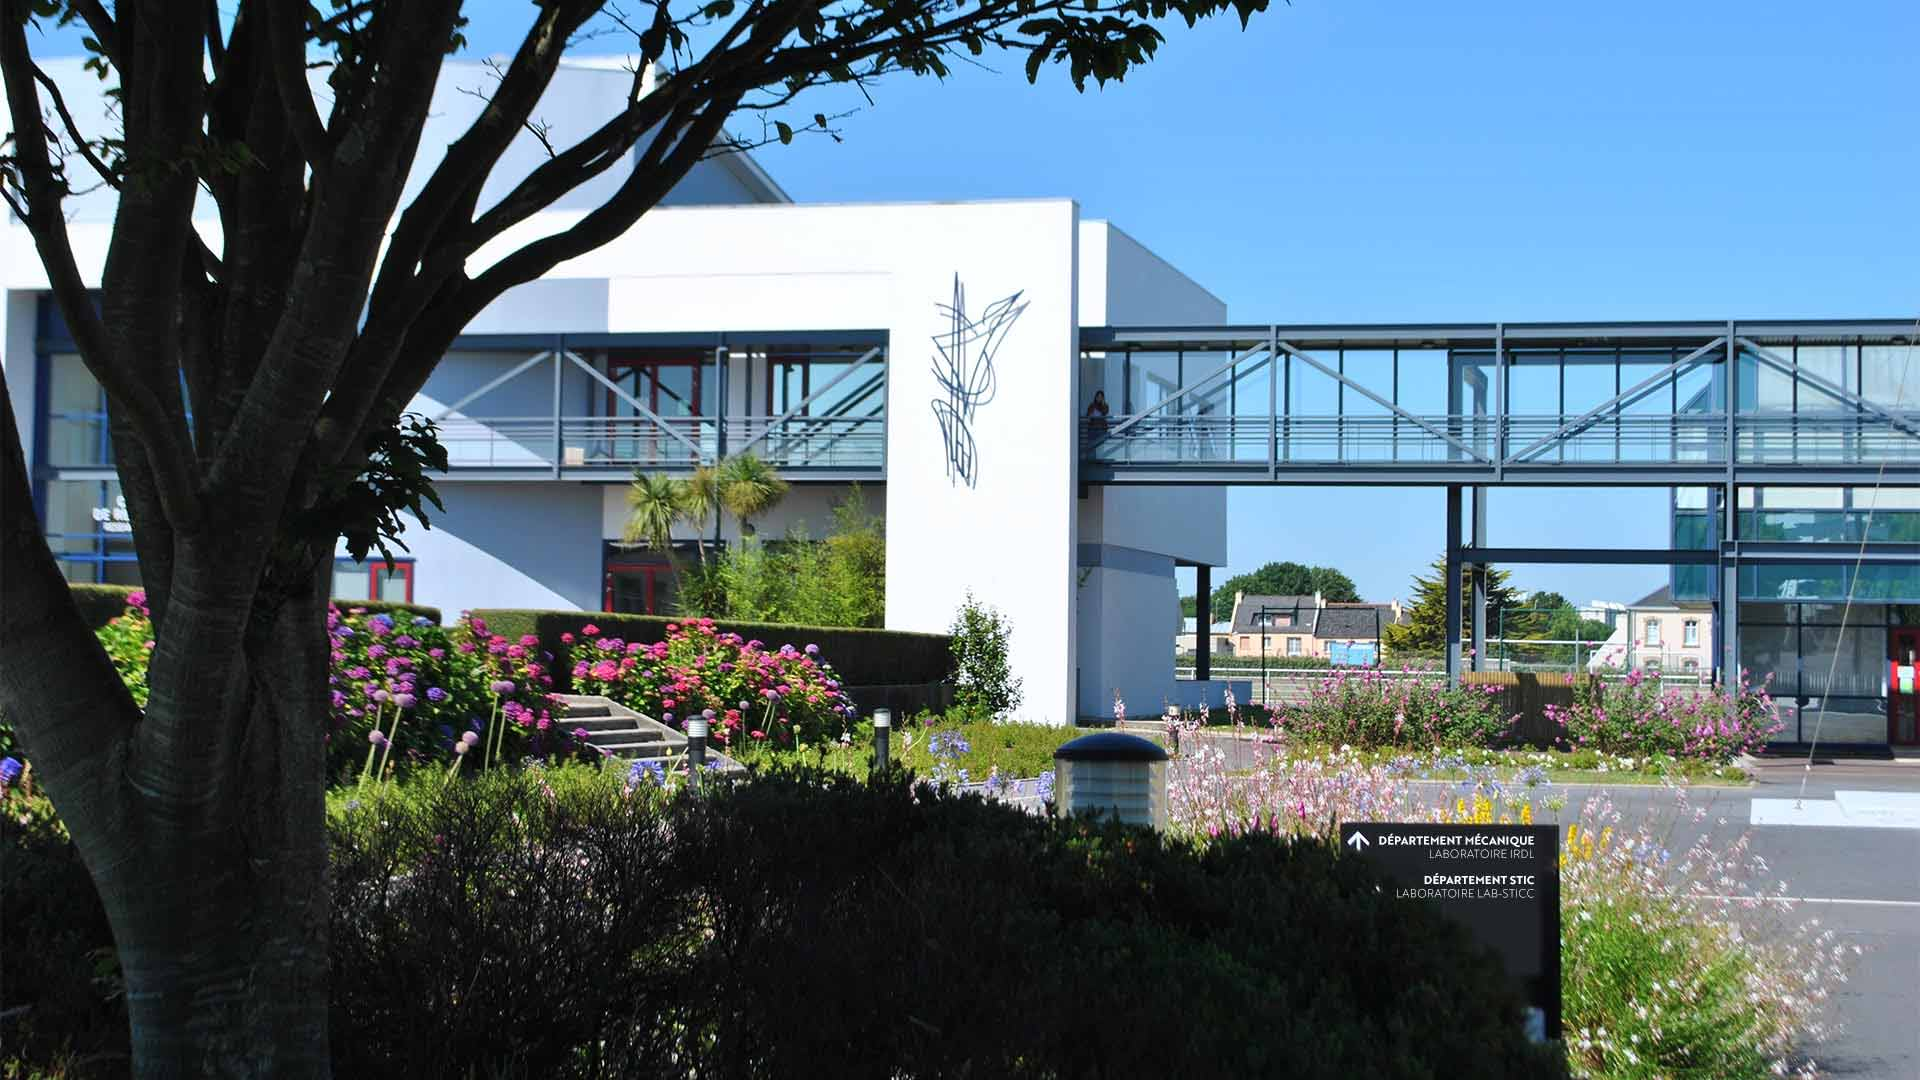
\includegraphics[height=0.7\textheight, trim={24cm 0 16cm 0}, clip]{images/ensta.jpg}
			\end{minipage}
		\end{frame}

	\part{Underwater acoustic propagation simulation using Finite Difference Time Domain}

		\begin{frame}
			\frametitle{Table of contents}
			\tableofcontents%[hideallsubsections]
		\end{frame}

		\section{Introduction}
		% \AllSectionsWithTitlePage

			\subsection{Scope of the study}

				\begin{frame}{Introduction}{Scope of the study}
					\centering
					\begin{minipage}{0.6\textwidth}
						\begin{block}{Variables of interest}
							\begin{itemize}
								\item Pressure
								\item Particle velocity
							\end{itemize}
						\end{block}
						\begin{block}{Scope of the simulation}
							\begin{itemize}
								\item Rectilinear Grid support for fields
								\item Linear acoustic approximation
								\item Viscoelastic modeling of materials
							\end{itemize}
						\end{block}
					\end{minipage}
				\end{frame}

			\subsection{Wave equation}

				\begin{frame}{Introduction}{Wave Equation}
					\centering
					\begin{minipage}[c]{0.3\textwidth}
						\begin{figure}
							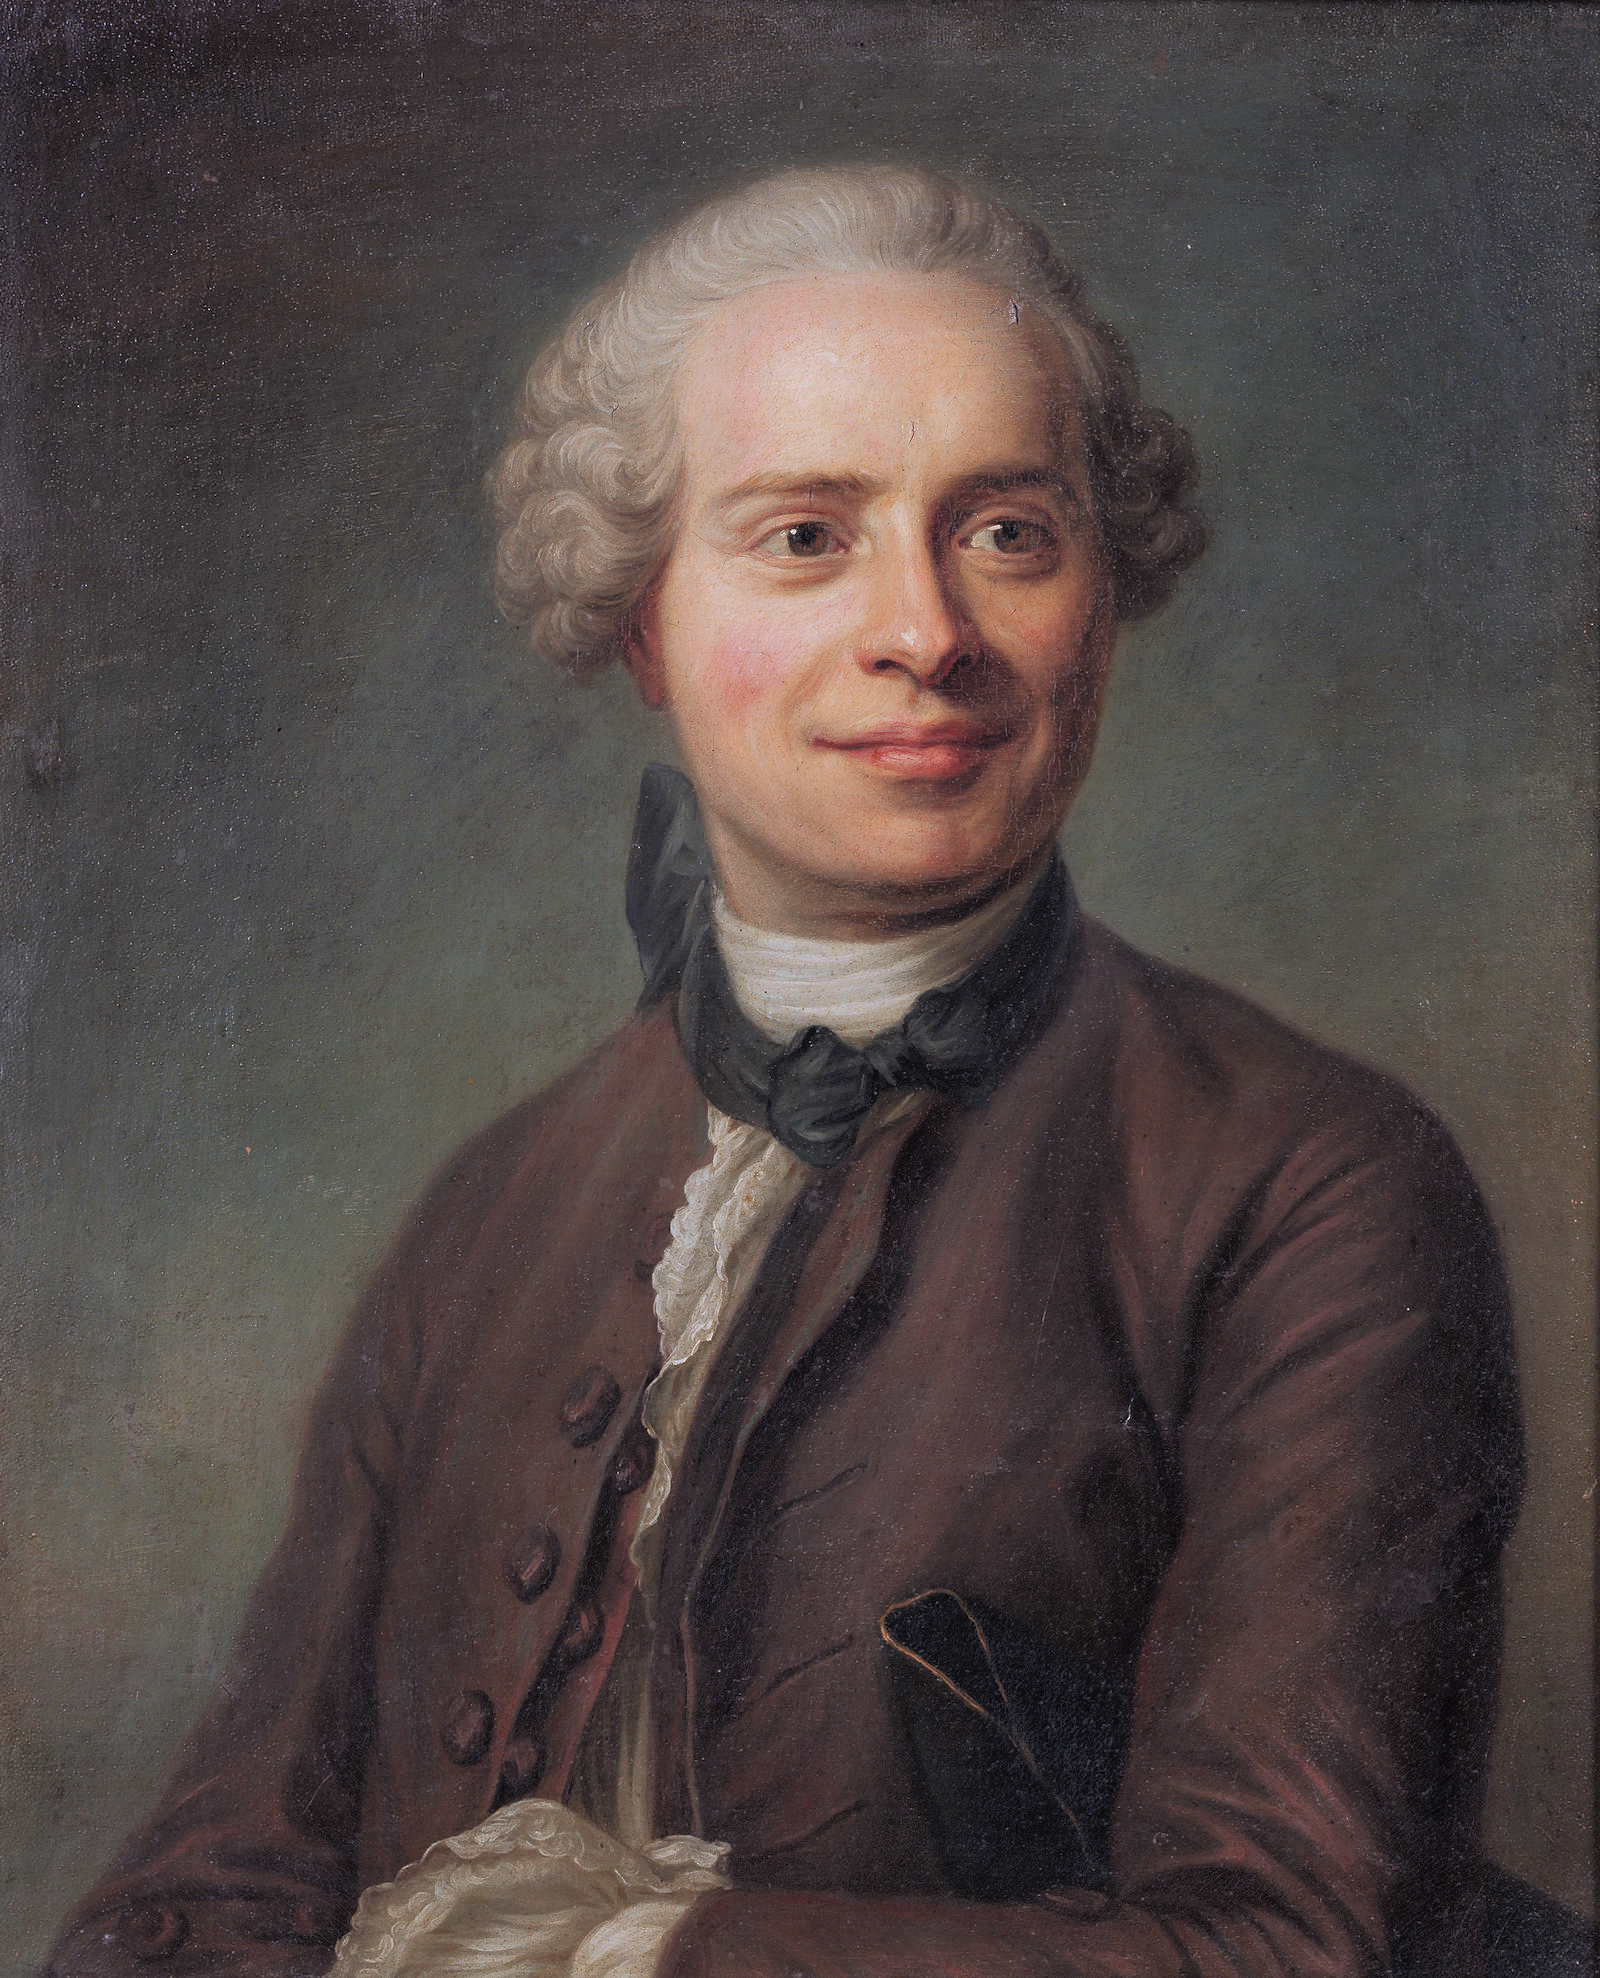
\includegraphics[width=\textwidth]{images/profile/Jean_Le_Rond_d'Alembert,_by_French_school.jpg}
							\caption{Jean Le Rond d'Alembert}
						\end{figure}
					\end{minipage}
					\hfill
					\begin{minipage}[c]{0.6\textwidth}
						\begin{alertblock}{Wave equation}
							\begin{eqnarray}
								\left(\nabla^2 - \frac{1}{c^2} \frac{\partial^2}{\partial t^2} \right) \phi(\mathbf{r}, t) & = & f(\mathbf{r}, t) \label{equation:alembert}
							\end{eqnarray}
							\begin{itemize}
								\item $\mathbf{r}$ : position
								\item $t$ : time
								\item $\phi$ : field
								\item $c$ : celerity 
							\end{itemize}
						\end{alertblock}
					\end{minipage}
				\end{frame}

		\section{Finite Difference Time Domain (FDTD)}

			\subsection{Numeric Scheme}

				\begin{frame}{FDTD}{Formalism}
					\centering
					\begin{minipage}[c]{0.45\textwidth}
						\begin{block}{Variables of interest}
							\begin{itemize}
								\item Pressure $p(t, x)$ \\
								\item Particle Velocity $u(t, x)$
							\end{itemize}
						\end{block}
						\begin{block}{Numeric scheme}
							\begin{itemize}
								\item $2^{nd}$ order in time $\mathcal{O}(\Delta t^2)$~\cite{blacnh1994FDTD} \\
								\item $4^{th}$ order in space $\mathcal{O}(\Delta x^4)$~\cite{blacnh1994FDTD}
							\end{itemize}
						\end{block}

						\onslide<2->{
							\begin{alertblock}{Staggered scheme}
								\only<2>{
								\begin{equation}
									\nabla p|_{i+\frac{1}{2}}^n = \frac{p|_{i+1}^n - p|_i^n}{\Delta x}
								\end{equation}}
								\only<3>{
								\begin{equation}
									\frac{\partial u}{\partial t}|_{i+\frac{1}{2}}^n = \frac{u|_{i+\frac{1}{2}}^{n+\frac{1}{2}} - u|_{i+\frac{1}{2}}^{n-\frac{1}{2}}}{\Delta t}
								\end{equation}}
								\only<4>{
									\begin{equation}
										\nabla p|_{i+\frac{1}{2}}^n = \rho \frac{\partial u}{\partial t}|_{i+\frac{1}{2}}^n
									\end{equation}
								}
							\end{alertblock}
						}
					\end{minipage}
					\hfill
					\begin{minipage}[c]{0.45\textwidth}
						\begin{figure}[!htb]
							\centering
							\resizebox{0.8\textwidth}{!}{
								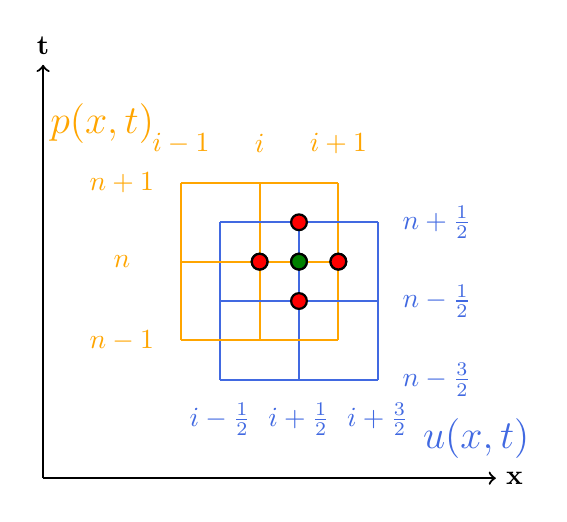
\begin{tikzpicture}
									\foreach \i in {-1,...,1} {
										\draw [Orange, thick] (\i,-1) -- (\i,1);
										\draw [RoyalBlue, thick] (\i+0.5,-1.5) -- (\i+0.5,0.5);
									}
									\foreach \i in {-1,...,1} {
										\draw [Orange, thick] (-1,\i) -- (1,\i);
										\draw [RoyalBlue, thick] (-0.5,\i-0.5) -- (1.5,\i-0.5);
									}
									\node[Orange] at (-2, 1.75) {\Large{$p(x, t)$}};
									\node[RoyalBlue] at (2.75, -2.25) {\Large{$u(x, t)$}};
					
									\node[Orange] at (-1.75, 1) {\normalsize{$n+1$}};
									\node[Orange] at (-1.75, 0) {\normalsize{$n$}};
									\node[Orange] at (-1.75, -1) {\normalsize{$n-1$}};
									\node[Orange] at (1, 1.5) {\normalsize{$i+1$}};
									\node[Orange] at (0, 1.5) {\normalsize{$i$}};
									\node[Orange] at (-1,1.5) {\normalsize{$i-1$}};
					
									\node[RoyalBlue] at (2.25, 0.5) {\normalsize{$n+\frac{1}{2}$}};
									\node[RoyalBlue] at (2.25, -0.5) {\normalsize{$n-\frac{1}{2}$}};
									\node[RoyalBlue] at (2.25, -1.5) {\normalsize{$n-\frac{3}{2}$}};
									\node[RoyalBlue] at (1.5, -2) {\normalsize{$i+\frac{3}{2}$}};
									\node[RoyalBlue] at (0.5, -2) {\normalsize{$i+\frac{1}{2}$}};
									\node[RoyalBlue] at (-0.5, -2) {\normalsize{$i-\frac{1}{2}$}};

									\draw[-to, >=latex, thick] (-2.75,-2.75) -- (3, -2.75) node[right] {$\mathbf{x}$};
									\draw[-to, >=latex, thick] (-2.75,-2.75) -- (-2.75, 2.5) node[above] {$\mathbf{t}$};

									\draw[thick, black, fill=Red, visible on=<2-2>] (0,0) circle (0.1);
									\draw[thick, black, fill=Red, visible on=<2-2>] (1,0) circle (0.1);
									\draw[thick, black, fill=Green, visible on=<2-2>] (0.5,0) circle (0.1);

									\draw[thick, black, fill=Red, visible on=<3-4>] (0.5,-0.5) circle (0.1);
									\draw[thick, black, fill=Red, visible on=<3-4>] (0.5,0.5) circle (0.1);
									\draw[thick, black, fill=Green, visible on=<3-4>] (0.5,0) circle (0.1);

									\draw[thick, black, fill=Red, visible on=<4>] (0,0) circle (0.1);
									\draw[thick, black, fill=Red, visible on=<4>] (1,0) circle (0.1);
							\end{tikzpicture}}
							\caption{Staggered pressure and particle velocity fields}
							\label{fig:staggered}
						\end{figure}
					\end{minipage}
				\end{frame}

			\subsection{Viscoelastic modeling of materials}

				\begin{frame}{FDTD}{Viscoelastic modeling of materials}
					\centering
					\begin{minipage}[c]{0.3\textwidth}
						\begin{figure}
							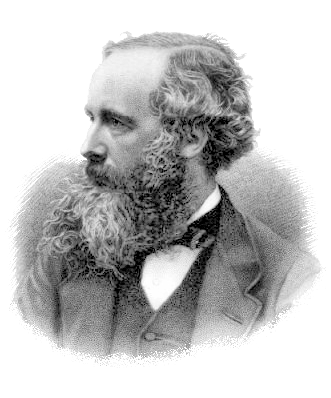
\includegraphics[width=\textwidth]{images/profile/James_Clerk_Maxwell.png}
							\caption{James Clerk Maxwell}
						\end{figure}
					\end{minipage}
					\hfill
					\begin{minipage}[c]{0.6\textwidth}
						\begin{block}{Standard Linear Solid model}
							\begin{itemize}
								\item Viscoelastic material modeling 
								\item Springs
								\item Dashpots
							\end{itemize}
						\end{block}
						\begin{figure}
							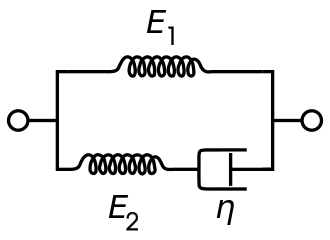
\includegraphics[width=0.4\textwidth]{images/SLS.png}
							\caption{Standard Linear Solid model, Maxwell representation}
						\end{figure}
					\end{minipage}
				\end{frame}

				\begin{frame}{FDTD}{Viscoelastic modeling of materials}
					\begin{minipage}[t]{0.48\textwidth}

						\begin{alertblock}{Q modeling}
							\begin{equation}
								Q^{-1}(\omega) \approx \sum_{l=1}^L \frac{\omega \tau_{\sigma l} \tau}{1 + \omega^2\tau_{\sigma l}^2}
							\end{equation}
							\begin{itemize}
								\item $Q$ : Desired quality factor 
								\item $\omega$ Pulsation
								\item $L$ : Number of SLS
								\item $\tau_{\sigma l}$ : Relaxation constraint
								\item $\tau$ : Computed constant for material
							\end{itemize}
						\end{alertblock}
					\end{minipage}
					\hfill
					\begin{minipage}[t]{0.48\textwidth}
						\begin{figure}
							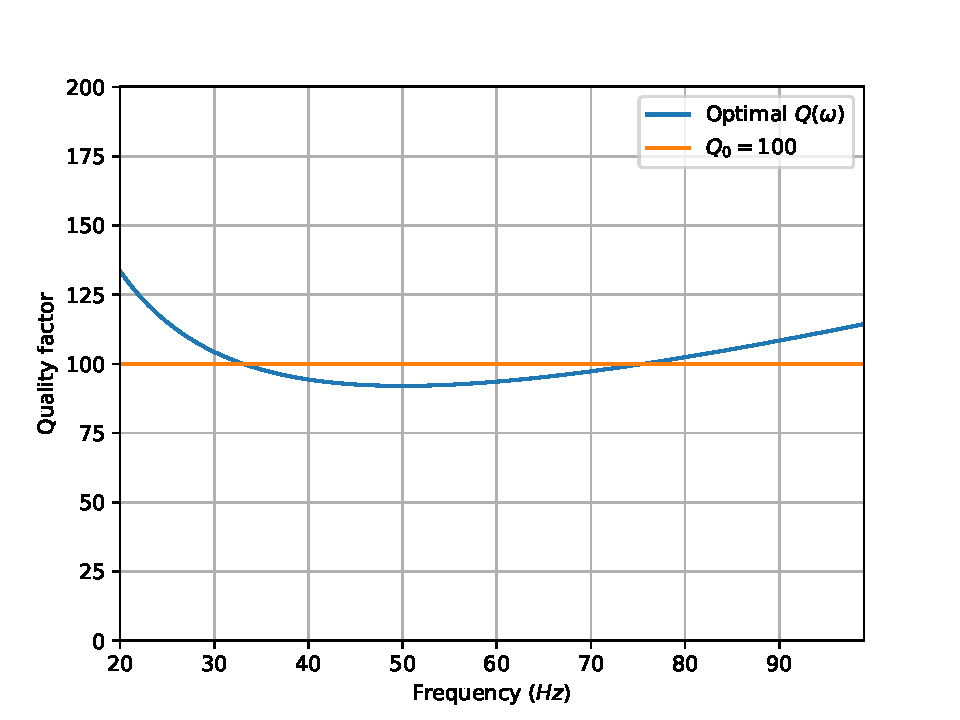
\includegraphics[width=\textwidth]{images/quality_factor.pdf}
							\caption{Optimal quality factor over a frequency range}
						\end{figure}
					\end{minipage}
				\end{frame}

			\subsection{Physically constrained acoustic sources model}

		\section{Results}
			
			\subsection{Validation}

			\subsection{Pulsing sphere}

				\begin{frame}{Results}{Pulsing sphere}
					\centering
					\begin{minipage}[c]{0.45\textwidth}
						\begin{figure}
							\movie{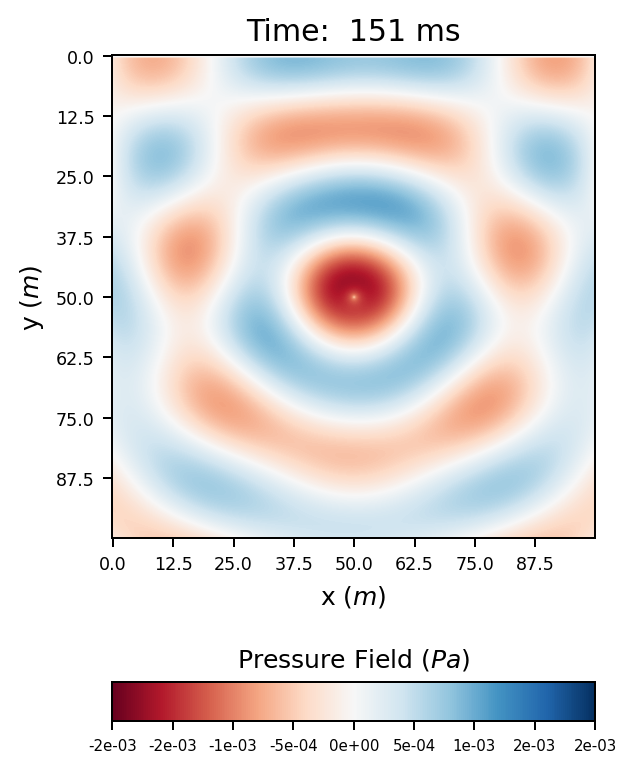
\includegraphics[width=\textwidth]{images/sphere/2dfdtd_00150.png}}{sphere.mp4}
						\end{figure}
					\end{minipage}
					\hfill
					\begin{minipage}[c]{0.5\textwidth}
						\begin{exampleblock}{Pulsing sphere}
							\begin{itemize}
								\item $(100,\ 100)\ m$ scene
								\item Emitter at $(50,\ 50)\ m$
								\item Reflection at the top
							\end{itemize}
						\end{exampleblock}
					\end{minipage}
				\end{frame}

	\part{Localization}

	\section{Validation}

		\subsection{Comparaison avec le modèle PyRAM}

			\begin{frame}{Scène}
				\begin{figure}[!htb]
					\centering
					\resizebox{0.8\textwidth}{!}{
					\begin{tikzpicture}
						\coordinate (A) at (0,0);
						\coordinate (B) at (0,4);
						\coordinate (C) at (8,4);
						\coordinate (D) at (8,0);
		
						\fill[Apricot!80] (A) -- ($(A)!0.3!(B)$) -- ($(D)!0.3!(C)$) -- (D) -- cycle;
						\fill[ProcessBlue!40] ($(A)!0.3!(B)$) -- (B) -- (C) -- ($(D)!0.3!(C)$) -- cycle;
						\node at ($(A)!0.5!(D)+(0,0.55)$) {Sédiments};
						\node at ($(A)!0.5!(D)+(0,2.25)$) {Eau};
						\draw[fill=Red] ($(A)!0.75!(B)$)  arc (-90:90:0.18) -- cycle;
						\node at ($(A)!0.79!(B)+(1,0)$) {Source};
						\draw (A) -- (B) -- (C) -- (D) -- cycle;
		
						\draw[to-to,>=latex] ($(A)-(0,0.3)$) -- node[below] {$r$} ($(D)-(0,0.3)$) ;
						\draw[to-to,>=latex] ($(A)-(0.7,0)$) -- node[left] {$z$} ($(B)-(0.7,0)$);
						\draw[to-to,>=latex] ($(A)!0.8!(B)-(0.1,0)$) -- node[left] {$z_s$} ($(B)-(0.1,0)$);
						\draw[to-to,>=latex] ($(A)-(0.1,0)$) -- node[left] {$h$} ($(A)!0.3!(B)-(0.1,0)$);
					\end{tikzpicture}}
					\caption{Scène utilisée dans la comparaison}
					\label{fig:scene}
				\end{figure}
			\end{frame}

			\begin{frame}{Comparaison}
				\begin{figure}[!htb]
					\centering
					\begin{subfigure}[b]{0.46\textwidth}
						\centering
						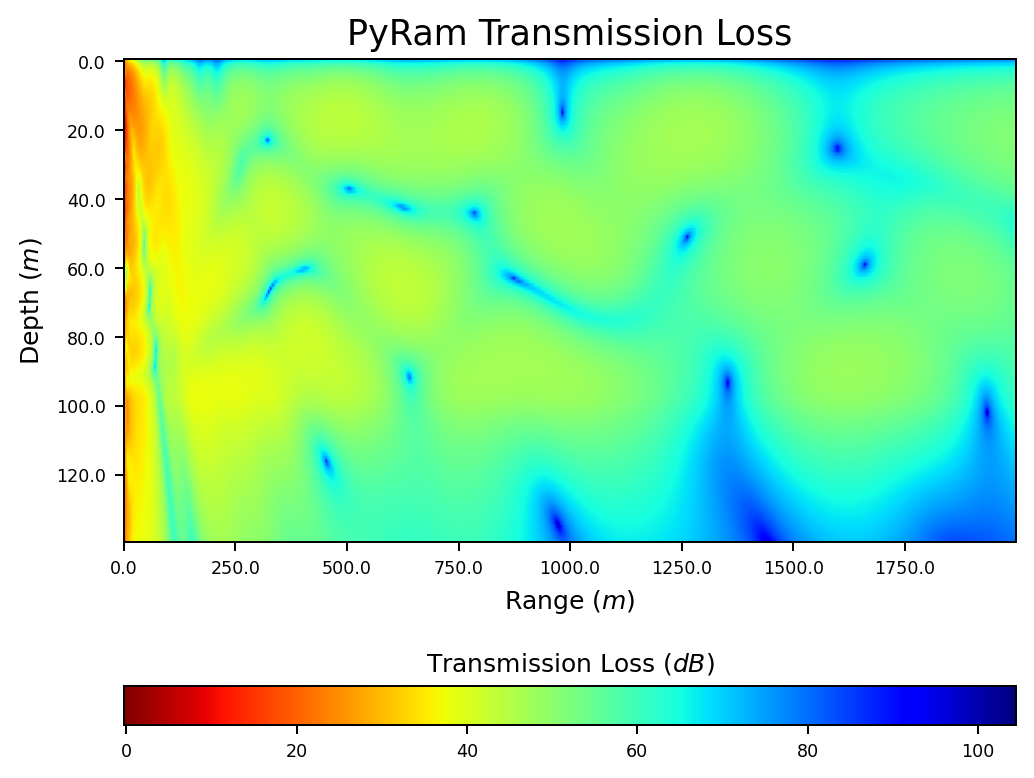
\includegraphics[width=\textwidth]{images/PyRam_Proteus.png}
						\caption{Modèle RAM}
						\label{fig:RAM}
					\end{subfigure}
					\hfill
					\begin{subfigure}[b]{0.49\textwidth}
						\centering
						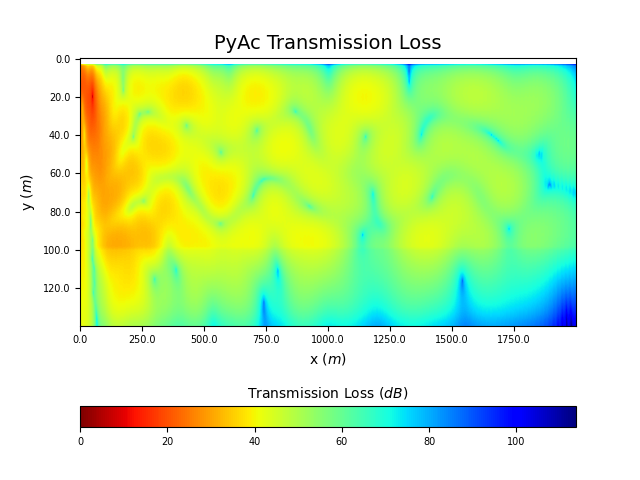
\includegraphics[width=\textwidth]{images/PyAc_Proteus_corrected.png}
						\caption{Modèle Différences Finies}
						\label{fig:FD}
					\end{subfigure}
					\caption{Comparaison des Transmission Loss simulées pour les deux modèles}
					\label{fig:comparison}
				\end{figure}
			\end{frame}

		\section{Localisation Ensembliste}

			\subsection{Méthodes Ensemblistes vs Probabilistes}

				\begin{frame}{Méthodes Ensembliste vs Probabilistes}
					\begin{minipage}[t]{0.45\textwidth}
						\begin{block}{Méthodes ensemblistes}
							\begin{itemize}
								\item Basées sur les ensembles
								\item Renvoie l'ensemble des possibilités
								\item Calcul garanti
							\end{itemize}
						\end{block}
						\begin{exampleblock}{Caractéristiques}
							\begin{itemize}
								\item Post-traitement
								\item Ensemble de solutions compatibles
								\item Domaine non-linéaires
							\end{itemize}
						\end{exampleblock}
					\end{minipage}
					\hfill
					\begin{minipage}[t]{0.45\textwidth}
						\begin{block}{Méthodes Probabilistes}
							\begin{itemize}
								\item Basées sur les probabilités
								\item Renvoie une position possible
								\item Calcul probable
							\end{itemize}
						\end{block}
						\begin{exampleblock}{Caractéristiques}
							\begin{itemize}
								\item Traitement temps réel
								\item Point avec covariance
								\item Domaine linéaire
							\end{itemize}
						\end{exampleblock}
					\end{minipage}
				\end{frame}

				\begin{frame}{Méthodes Ensembliste vs Probabilistes}
					\begin{minipage}[t]{0.45\textwidth}
						\begin{figure}
							\begin{tikzpicture}
								\tikzstyle{every node}=[font=\footnotesize]
								\coordinate (A) at (1.2,0);
								\coordinate (B) at (0,1);
								\coordinate (X) at ($(A)+(B)$);
								\draw[-to, >=latex] (0,0) -- ($(A)+(1,0)$);
								\draw[-to, >=latex] (0,0) -- ($(B)+(0,1)$);
								\filldraw[fill=Cerulean!20,draw=Cerulean!50] ($(X)+(0.512,0.491)$) rectangle ($(X)-(0.55,0.5)$);
								\node[Cerulean] at ($(X)-(0.7,0.7)$) {$[f](x)$};
								\node[ForestGreen] at ($(X)+(-0.7,0.7)$) {$f(x)$};
								\path[draw,use Hobby shortcut,closed=true,fill=ForestGreen!20,draw=ForestGreen!50] ($(X)-(0,0.5)$) .. ($(X)-(0.5,0.15)$) .. ($(X)+(0,0.4)$) .. ($(X)+(0.2,0.15)$) .. ($(X)+(0.3,+0.15)$);
								\filldraw[Magenta] (X) circle (0.05) node[above right, Magenta] {$x$};
								\node[below left] at (0, 0) {$O$};
								\node[below left] at ($(X)+(1,1)$) {$\mathbb{R}^n$};
							\end{tikzpicture}
							\caption{Méthodes ensemblistes}
						\end{figure}
						\begin{exampleblock}{Example}
							\begin{itemize}
								\item Intervalles
								\item Zonotopes
								\item Polytopes
							\end{itemize}
						\end{exampleblock}
					\end{minipage}
					\hfill
					\begin{minipage}[t]{0.45\textwidth}
						\begin{figure}
							\tikzstyle{every node}=[font=\footnotesize]
							\begin{tikzpicture}
								\coordinate (A) at (1.2,0);
								\coordinate (B) at (0,1);
								\coordinate (X) at ($(A)+(B)$);
								\draw[-to, >=latex] (0,0) -- ($(A)+(1,0)$);
								\draw[-to, >=latex] (0,0) -- ($(B)+(0,1)$);
								\filldraw[rotate=-33,fill=ForestGreen!20,draw=ForestGreen!50] ($(X)-(0.2,0.25)$) ellipse (12pt and 20pt);
								\filldraw[ForestGreen] ($(X)-(0.28,0.1)$) circle (0.05) node[below left, ForestGreen] {$\hat{x}$};
								\node[above left, ForestGreen] at ($(X)+(-0.35,0.25)$) {$\Gamma_x$};
								\filldraw[Magenta] (X) circle (0.05) node[above right, Magenta] {$x$};
								\node[below left] at (0, 0) {$O$};
								\node[below left] at ($(X)+(1,1)$) {$\mathbb{R}^n$};
							\end{tikzpicture}
							\caption{Méthodes probabilistes}
						\end{figure}
						\begin{exampleblock}{Example}
							\begin{itemize}
								\item Filtre de Kalman
								\item Filtre de Bayes
								\item Méthodes de Monte-Carlo
							\end{itemize}
						\end{exampleblock}
					\end{minipage}
				\end{frame}
				
			% 	\begin{frame}{Analyse par Intervalle}
			% 		\begin{block}{Formalisme}
			% 			Considérons la fonction :
			% 			\begin{align*}
			% 				f \colon \mathbb{R}^n \times \mathbb{R}^p &\to \mathbb{R}^n\\
			% 				(x \times y) &\mapsto f(x, y).
			% 			\end{align*}
			% 			$$\forall [x] \in \mathbb{R}^n, \quad \forall [y] \in \mathbb{R}^p, \quad \mathbb{X} = \left\{x \in [x],\; y \in [y],\; f(x, y) = 0 \right\}$$
			% 			en l'encadrant par deux sous-pavages $\mathbb{X}^-$ et $\mathbb{X}^+$ de $\mathbb{R}^m$ tels que :
			% 			\begin{equation*}
			% 				\mathbb{X}^- \subset \mathbb{X} \subset \mathbb{X}^+
			% 			\end{equation*}
			% 		\end{block}
			% 	\end{frame}
				
			% 	\begin{frame}{Contracteur}
			% 		\begin{block}{Contracteur}
			% 			L'opérateur $\mathcal{C} \colon \mathbb{R}^n \to \mathbb{R}^n$ est un contracteur pour $f(x) = 0$ si
			% 			\begin{empheq}[left=\empheqlbrace]{align*}
			% 				\; & \mathcal{C}([x]) \subset [x] & (Contractance) \\
			% 			\; & \mathcal{C}([x]) \cap \mathbb{X} = [x] \cap \mathbb{X} & (Completeness) \\
			% 			\; & (x \in [x]) \wedge (f(x) = 0) \; \Rightarrow \; (x \in \mathcal{C}([x])) & (Consistence)
			% 		\end{empheq}
			% 	\end{block}
			% \end{frame}


		\subsection{Localisation ensembliste de source acoustiques}

			\begin{frame}{Réciprocité Acoustique}
				\begin{minipage}{0.45\textwidth}
					\begin{block}{Réciprocité}
						\begin{itemize}
							\item Récepteurs $\leftrightarrow$ Émetteurs
							\item Carte de niveau acoustique perçus par rapport à un récepteur
							\item Résoudre problème d'inversion
						\end{itemize}
					\end{block}
					\begin{block}{Réciprocité Acoustique}
						\begin{itemize}
							\item Cadre de l'acoustique linéaire~\cite{rayleigh1896theory}
							\item Valable en avec modélisation visco-élastique des matériaux
						\end{itemize}
					\end{block}
				\end{minipage}
				\hfill
				\begin{minipage}{0.45\textwidth}
					\begin{figure}
						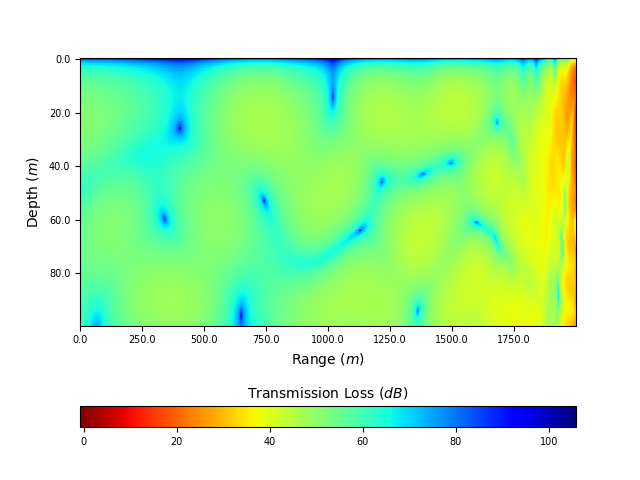
\includegraphics[width=\textwidth]{images/Reciever_20_2000.png}
						\caption{Carte de niveaux acoustiques pour un récepteur placé en $(2000, 20)\ m$}
					\end{figure}
				\end{minipage}
			\end{frame}

			\begin{frame}{Problème d'inversion}
				\begin{figure}[!htb]
					\begin{subfigure}[!htb]{\textwidth}
						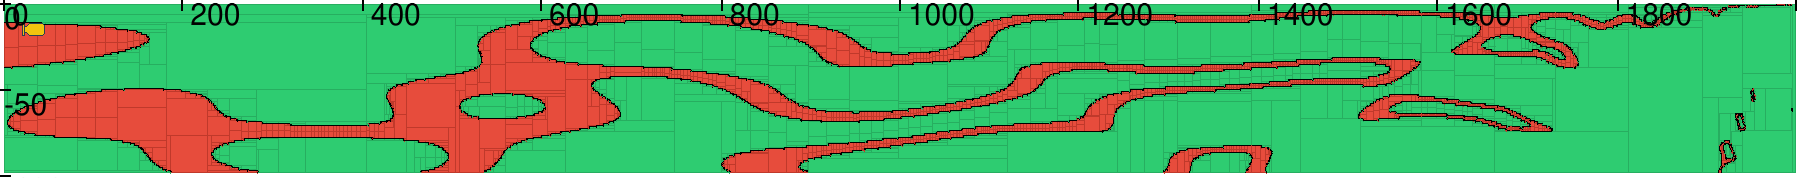
\includegraphics[width=\textwidth]{images/Hydrophone_20_2000.png}
						\caption{Compatibilité avec Hydrophone placé en $(2000, 20)\ m$}
					\end{subfigure}
					\begin{subfigure}[!htb]{\textwidth}
						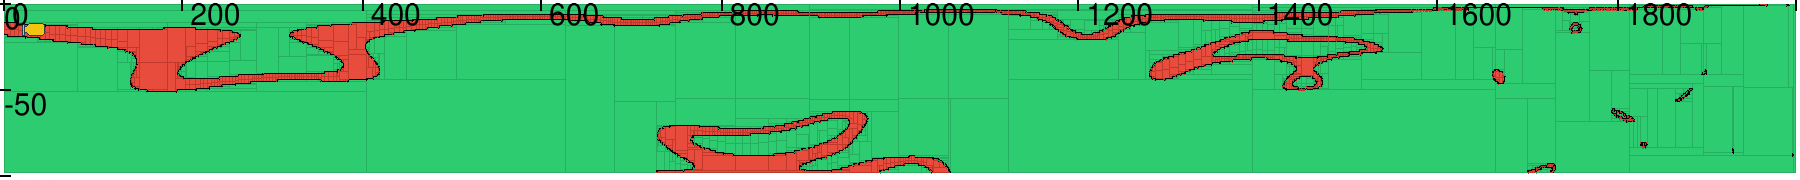
\includegraphics[width=\textwidth]{images/Hydrophone_40_2000.png}
						\caption{Compatibilité avec Hydrophone placé en $(2000, 40)\ m$}
					\end{subfigure}
					\begin{subfigure}[!htb]{\textwidth}
						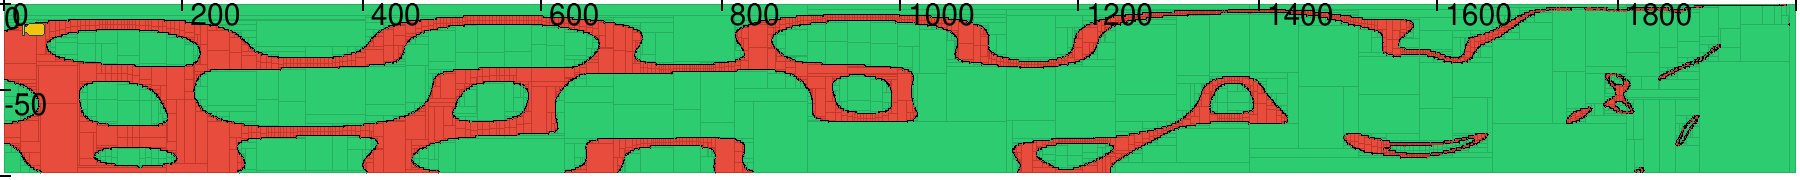
\includegraphics[width=\textwidth]{images/Hydrophone_60_2000.png}
						\caption{Compatibilité avec Hydrophone placé en $(2000, 60)\ m$}
					\end{subfigure}
					\begin{subfigure}[!htb]{\textwidth}
						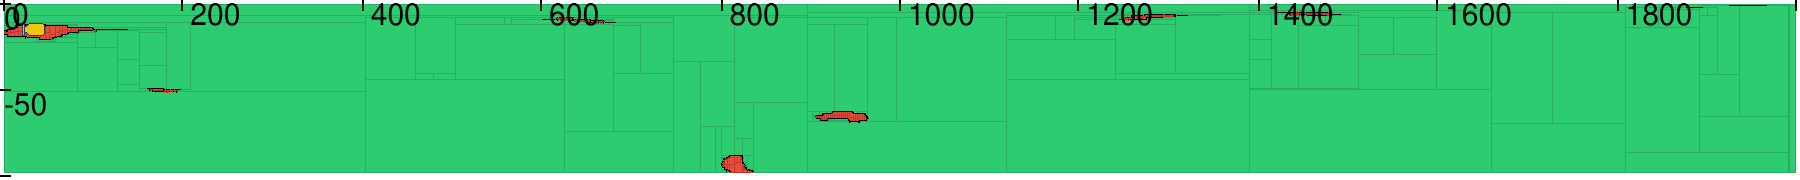
\includegraphics[width=\textwidth]{images/Proteus.png}
						\caption{Position de la source compatibles avec les mesures de niveaux acoustiques}
					\end{subfigure}
					\caption{Localisation ensembliste de la source acoustique}
				\end{figure}
			\end{frame}

		\section{Conclusion}
		
			\begin{frame}{Conclusion}
				\centering
				\begin{minipage}{0.55\textwidth}
					\begin{block}{Améliorations}
						\begin{itemize}
							\item Modélisation du bruit 
							\item Passage de la 2D à la 3D
							\item Passage du Python au C++
							\item Validation en milieu naturel
						\end{itemize}
					\end{block}

					\begin{block}{Localisation ensembliste}
						\begin{itemize}
							\item Émetteur/Récepteur en mouvement
							\item Simulation à plusieurs fréquences
							\item Navigation dans données sonar
							\item SLAM acoustique
						\end{itemize}
					\end{block}
				\end{minipage}
				\hfill
				\begin{minipage}{0.4\textwidth}
					\centering
					\begin{figure}
						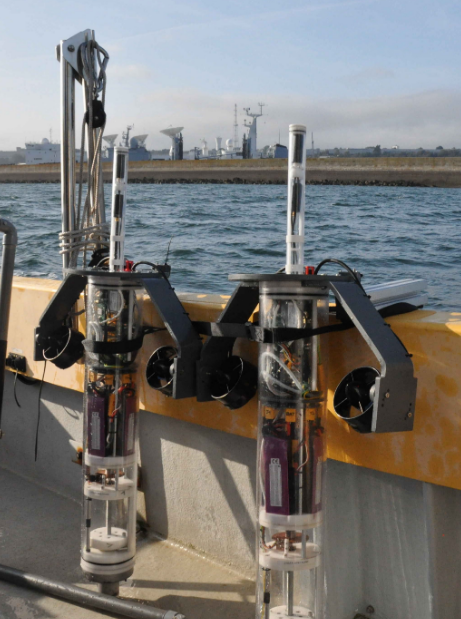
\includegraphics[width=0.8\textwidth]{images/seabot.png}
						\caption{SeaBot - Thomas Le Mézo}
					\end{figure}
				\end{minipage}
			\end{frame}
	
		\begin{frame}{Bibliographie}
			\bibliography{bib/presentation}
			\bibliographystyle{ieeetr}
		\end{frame}
\end{document}